\chapter{需求建模 }
\section{数据流图}
\subsection{顶层数据流图}
\iffalse
<Draw the Top-level DFD here>

在这里画出顶层数据流图
\fi
  \begin{figure}[!h]
  	\centering
	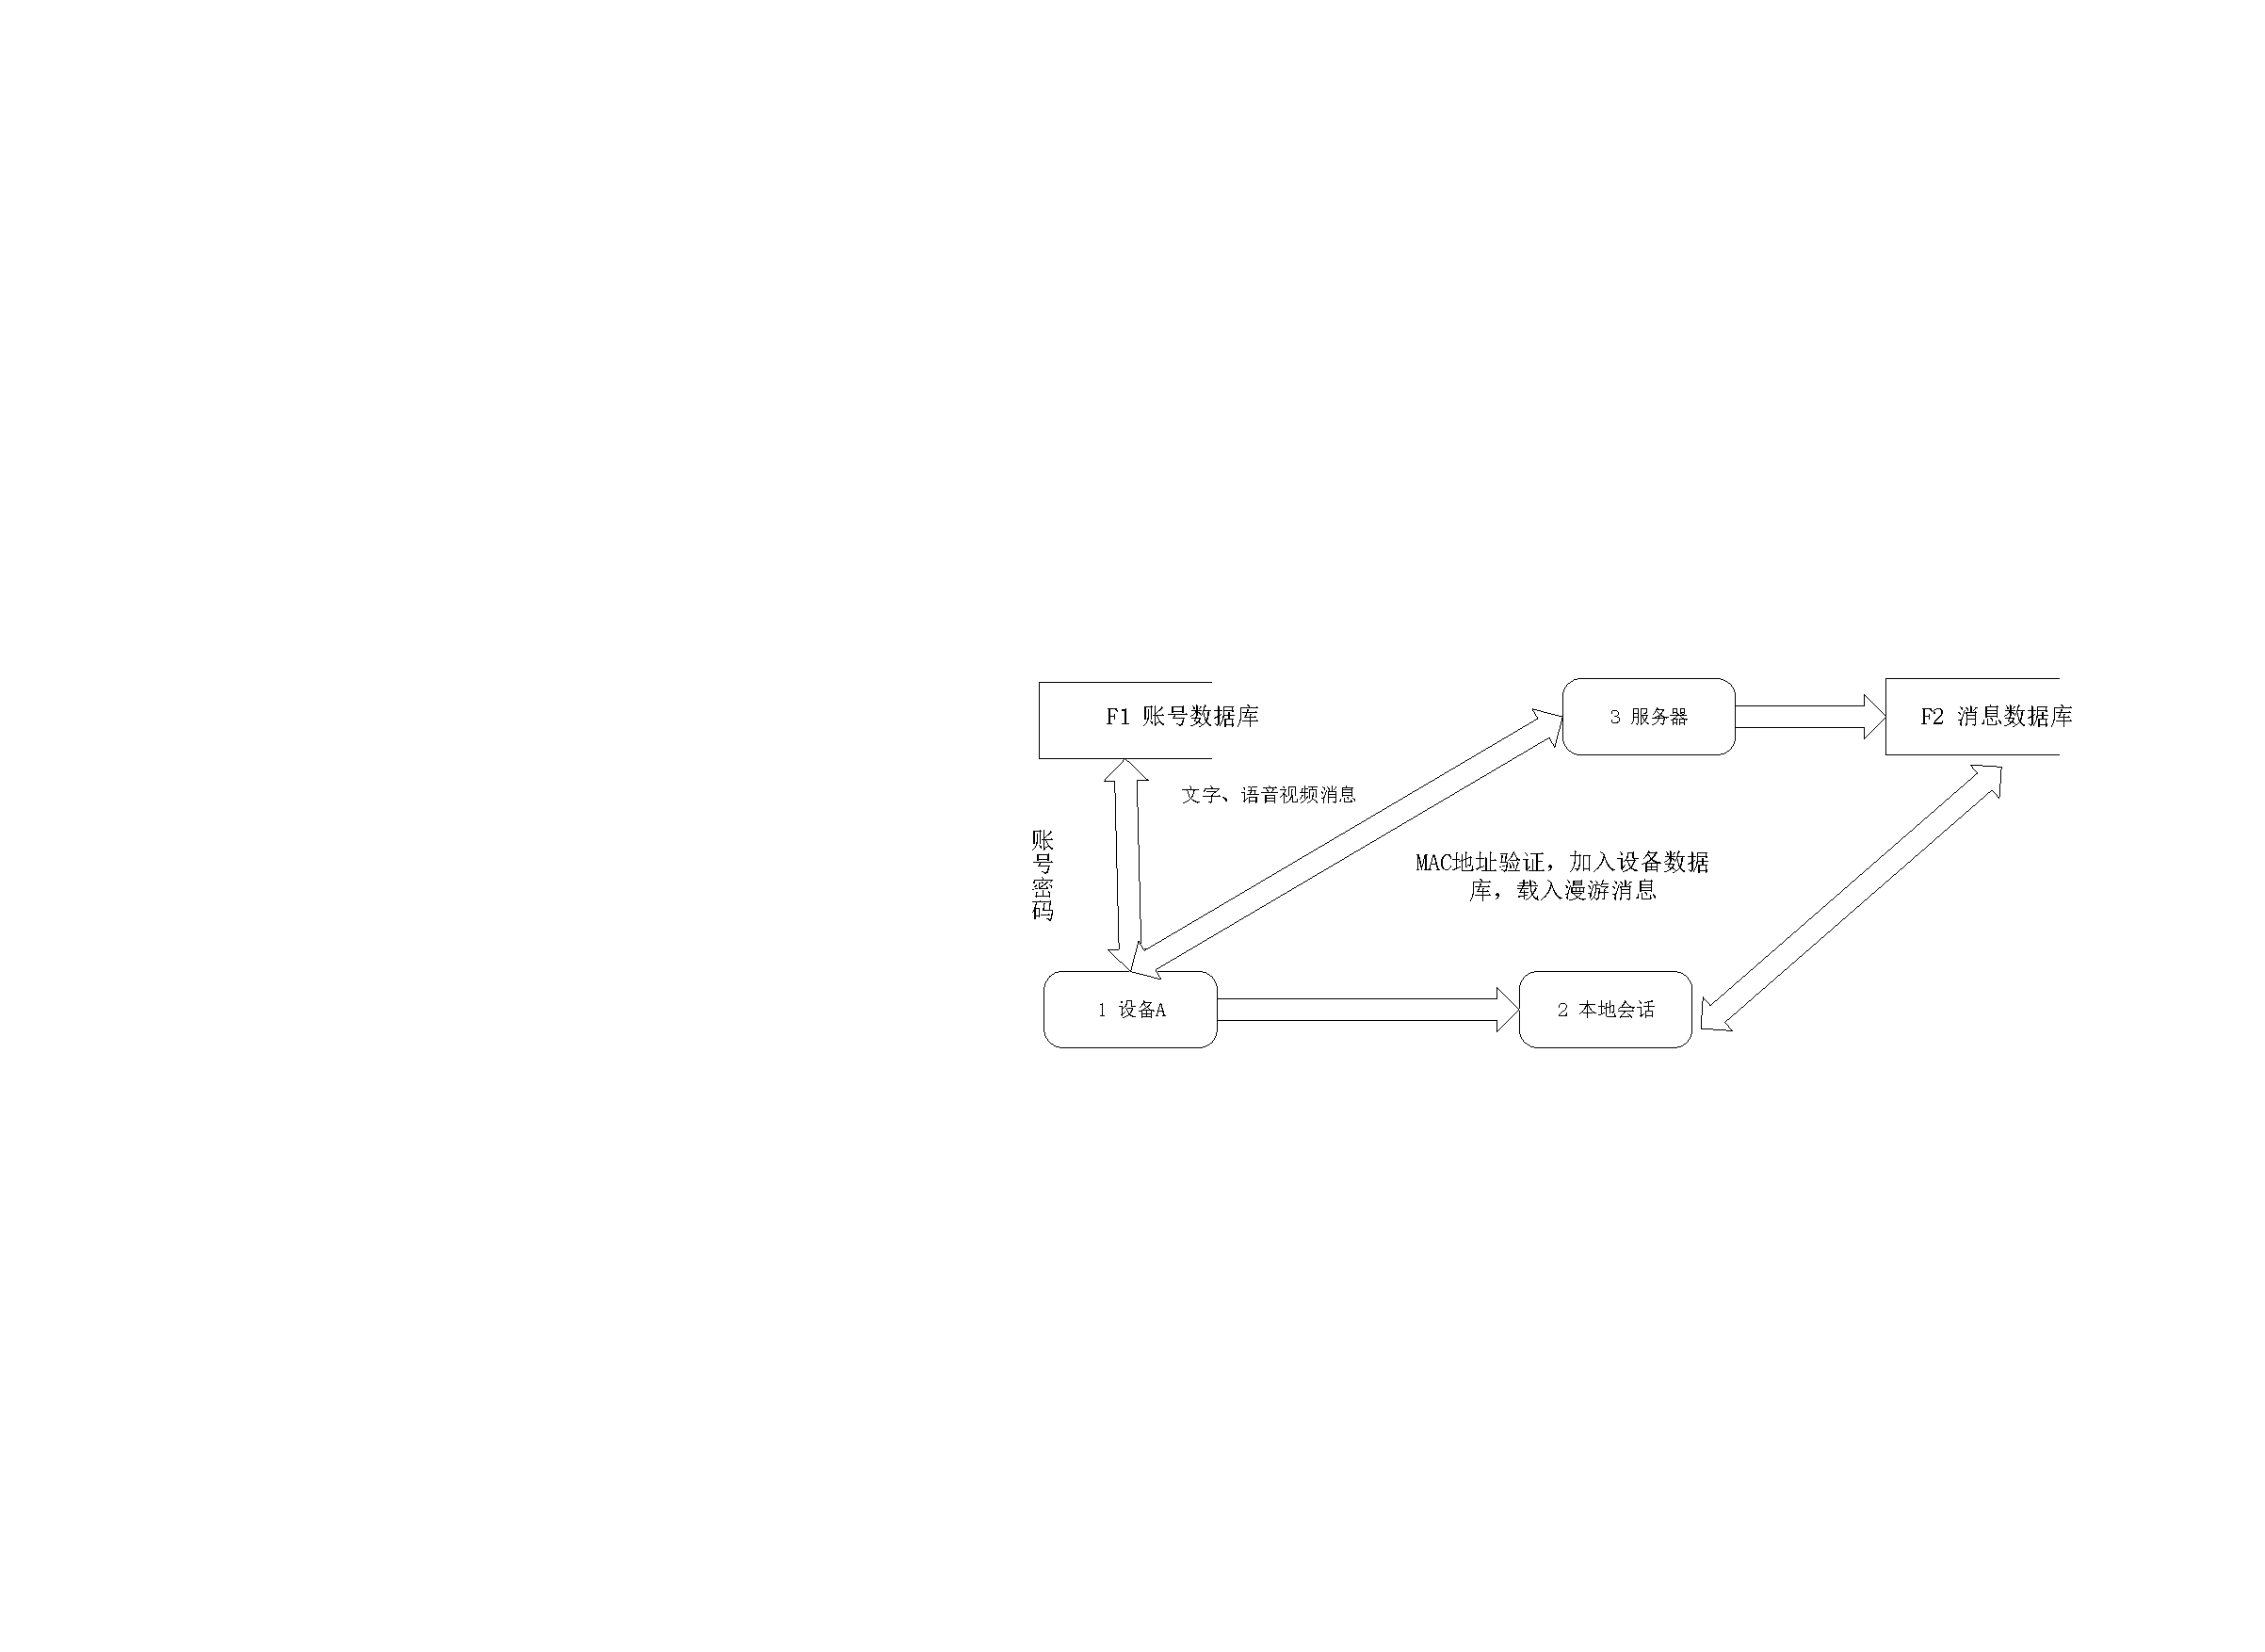
\includegraphics[width=11cm]{DFD}
	\note{顶层数据流图}
	\label{fig:noted-figure}
  \end{figure}
\subsection{层数据流图}
\iffalse
<Draw the Level-0 DFD here>

在这里画出0层数据流图
\fi
  \begin{figure}[!h]
  	\centering
	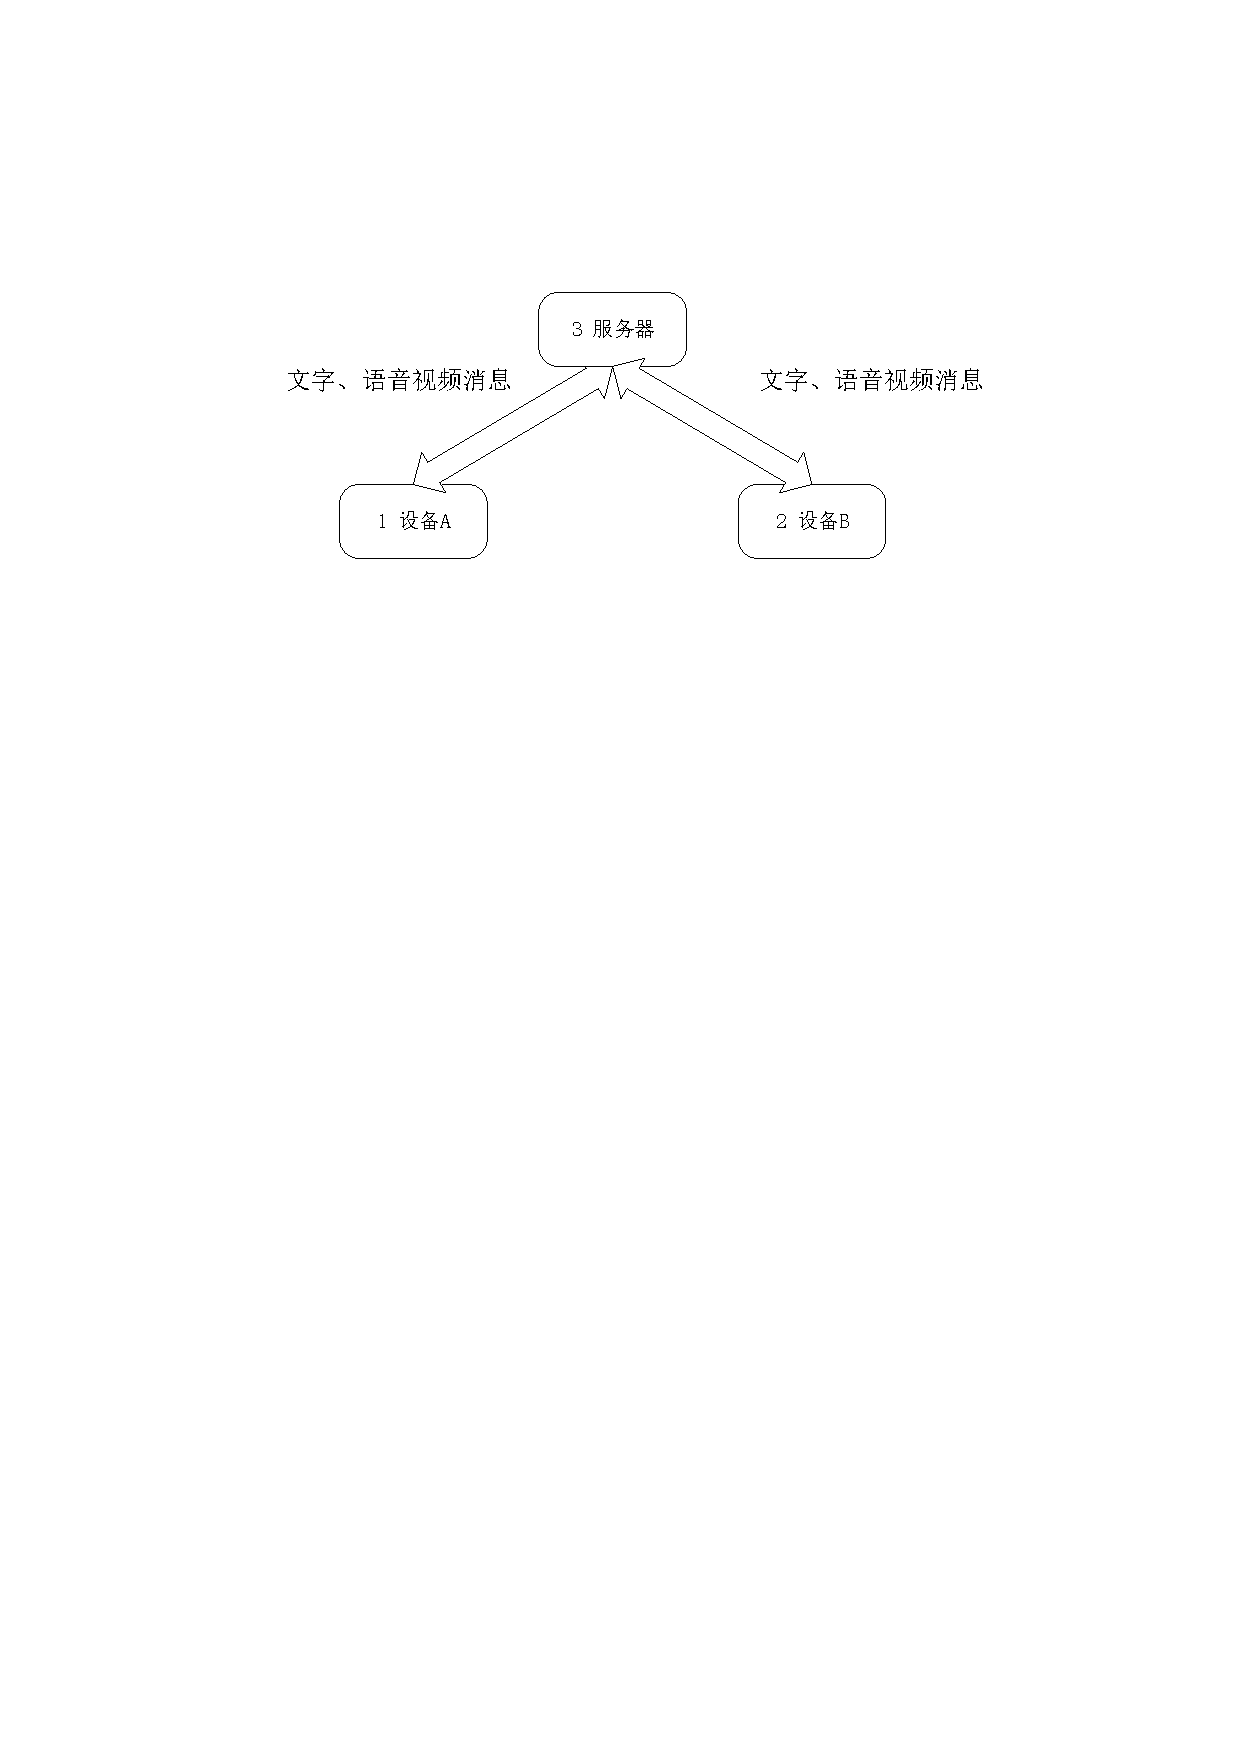
\includegraphics[width=11cm]{levelDFD}
	\note{层数据流图}
	\label{fig:noted-figure}
  \end{figure}

\section{数据字典}
\subsection{数据流说明}
\subsubsection{数据流1名称}
\iffalse
<Title of  the data flow should accord with the one in data flow diagram, and the Data description notions should be used.  >

与数据流图中的名称一致,采用数据描述符号说明数据流的内容
\fi
\subsubsection{数据流2名称}
\iffalse
<Title of  the data flow should accord with the one in data flow diagram, and the Data description notions should be used   >

与数据流图中的名称一致,采用数据描述符号说明数据流的内容
\fi
\subsection{数据存储说明}
\subsubsection{数据存储1名称}
\iffalse
<Title of  the data flow should accord with the one in data flow diagram, and the Data description notions should be used. The arrangement of the data in data store should also be described.>

与数据流图中的名称一致,采用数据描述符号说明数据流的内容,另外还需描述数据排列方式
\fi
F1为用户账号密码经过加密哈希后的数据库。为关系数据模型。数据排列方式为平铺排列。
\subsubsection{数据存储2名称}
\iffalse
<Title of  the data flow should accord with the one in data flow diagram, and the Data description notions should be used.The arrangement of the data in data store should also be described.>

与数据流图中的名称一致,采用数据描述符号说明数据流的内容,另外还需描述数据排列方式
\fi
F2 为用户会话消息数据库
为对象型数据模型,为每个用户对/用户群之间建立关系,将聊天历史文件加密后存储
\subsection{加工说明}
\subsubsection{加工1名称}
\iffalse
<Use natural language, Decision table/Decision tree and Pseudocode to describe how to process the data flow>

采用自然语言,判断表/判断树,伪码的形式描述对数据流进行处理的过程
\fi
处理过程:
账号密码进行加盐处理,并哈希后与F1中已有值比较。本地验证码验证。\\
设备向服务器发出HTTP报文的连接请求,服务器识别设备的mac地址,并将其加入信任列表\\
服务器想消息数据库发送请求,加载包含改用户的所有会话消息\\
服务器用所有会话消息更新设备\\
设备创建本地会话\\
本地会话间隔固定时间加密上传\\
